\frame[plain]{\titlepage}
% \frame{\frametitle{Outline}\tableofcontents}

% \section{Introduction}

% \begin{frame}
%     \frametitle{Introduction}
    
%     In the presentation, I would first introduce Monte Carlo Integration, which requires enormous random sample. Then we introduce common ways of sampling from a given distribution, including Transformation method, Accept-rejection method, and Markov Chain Monte Carlo Algorithm. In each method I would show code implementation, analyse the pros and cons, and a brief proof.
    
% \end{frame}
\section[MC Integration]{Monte Carlo Integration}
\begin{frame}
    \frametitle{MC Integration}
    Suppose we want to evaluate an integral
    \begin{align*}
    \int_D \phi(x) d x
    \end{align*}
    for which there is no closed analytic solution. If the integration has the form
    \begin{align*}
    \phi(x)=\tilde{\phi}(x) f(x)
    \end{align*}
    for some density function \(f\), then the integral has the form:
    \begin{align*}
    \int_D \phi(x) d x=\int_D \tilde{\phi}(x) f(x) d x=E[\tilde{\phi}(X)]
    \end{align*}
    where \(\mathrm{X}\) is an RV with \(\mathrm{PDF} f\). 

    

\end{frame}
\begin{frame}
    % \frametitle{<title>}
    \frametitle{MC Integration}
    If we know how to simulate realisations of \(X\), say \(x^{(1)}, \ldots, x^{(n)}\), then we have an estimate
    \begin{align*}
    \int_D \phi(x) d x=E[\tilde{\phi}(X)] \approx \frac{1}{n} \sum_{i=1}^n \tilde{\phi}\left(x^{(i)}\right)=\hat{I}
    \end{align*}
    \pause
    Also, the variance should be
    \begin{align*}
        \operatorname{Var}(I) &= \frac{1}{n^2} \sum_{i=1}^n \operatorname{Var}\left(\tilde{\phi}\left(x\right)\right) \\
        &\approx \frac{1}{n(n-1)} \sum_{i=1}^n \left(\tilde{\phi}\left(x^{(i)}\right) - \hat I\right)
    \end{align*}
    % \vspace{1em}
    So it is crucial to generate sample from a specific distribution.

    

\end{frame}
\section{Transformation method}
\subsection{Algorithm}

\begin{frame}
    \frametitle{Derivation of the Algorithm}

    The easiest distribution for computer to generate is \(\operatorname{Unif}[0,1]\). If \(X\) owns CDF \(F(\cdot)\), Then \(F(X) \sim \operatorname{Unif}[0.1]\). By \textit{inversion}, setting \(X \sim F^{-1}(U)\), which \(U \sim \operatorname{Unif}[0,1]\). Then From the uniform distribution sample we can generate sample follows \(F(\cdot)\).
    \vspace*{1em}

    \pause

    Consider discrete random variable, simply left
    \[F^{-1} (u) = \min\left\{x:F(x)\geq u\right\}\]
    And the algorithm goes on as continuous situation.

\end{frame}
\subsection{Pros and Cons}
\begin{frame}
    \frametitle{Pros and Cons}
    \begin{columns}
        \column{0.5\textwidth}
        \begin{block}{Pros}
            \begin{itemize}
                \item Naive way to generate a group of sample
                % \item ?
                \\
            \end{itemize}
        \end{block}
        
        \column{0.5\textwidth}
        \begin{block}{Cons}
            \begin{itemize}
                \item The CDF is not invertible,i.e. PDF \(f(\cdot) = 0\) somewhere.
            \end{itemize}
        \end{block}

        
    \end{columns}
    
\end{frame}
\section{Accept-Reject method}
\subsection{Intuition}

\begin{frame}
    \frametitle{Intuition}

    % require graph
    \begin{figure}
        \begin{center}
            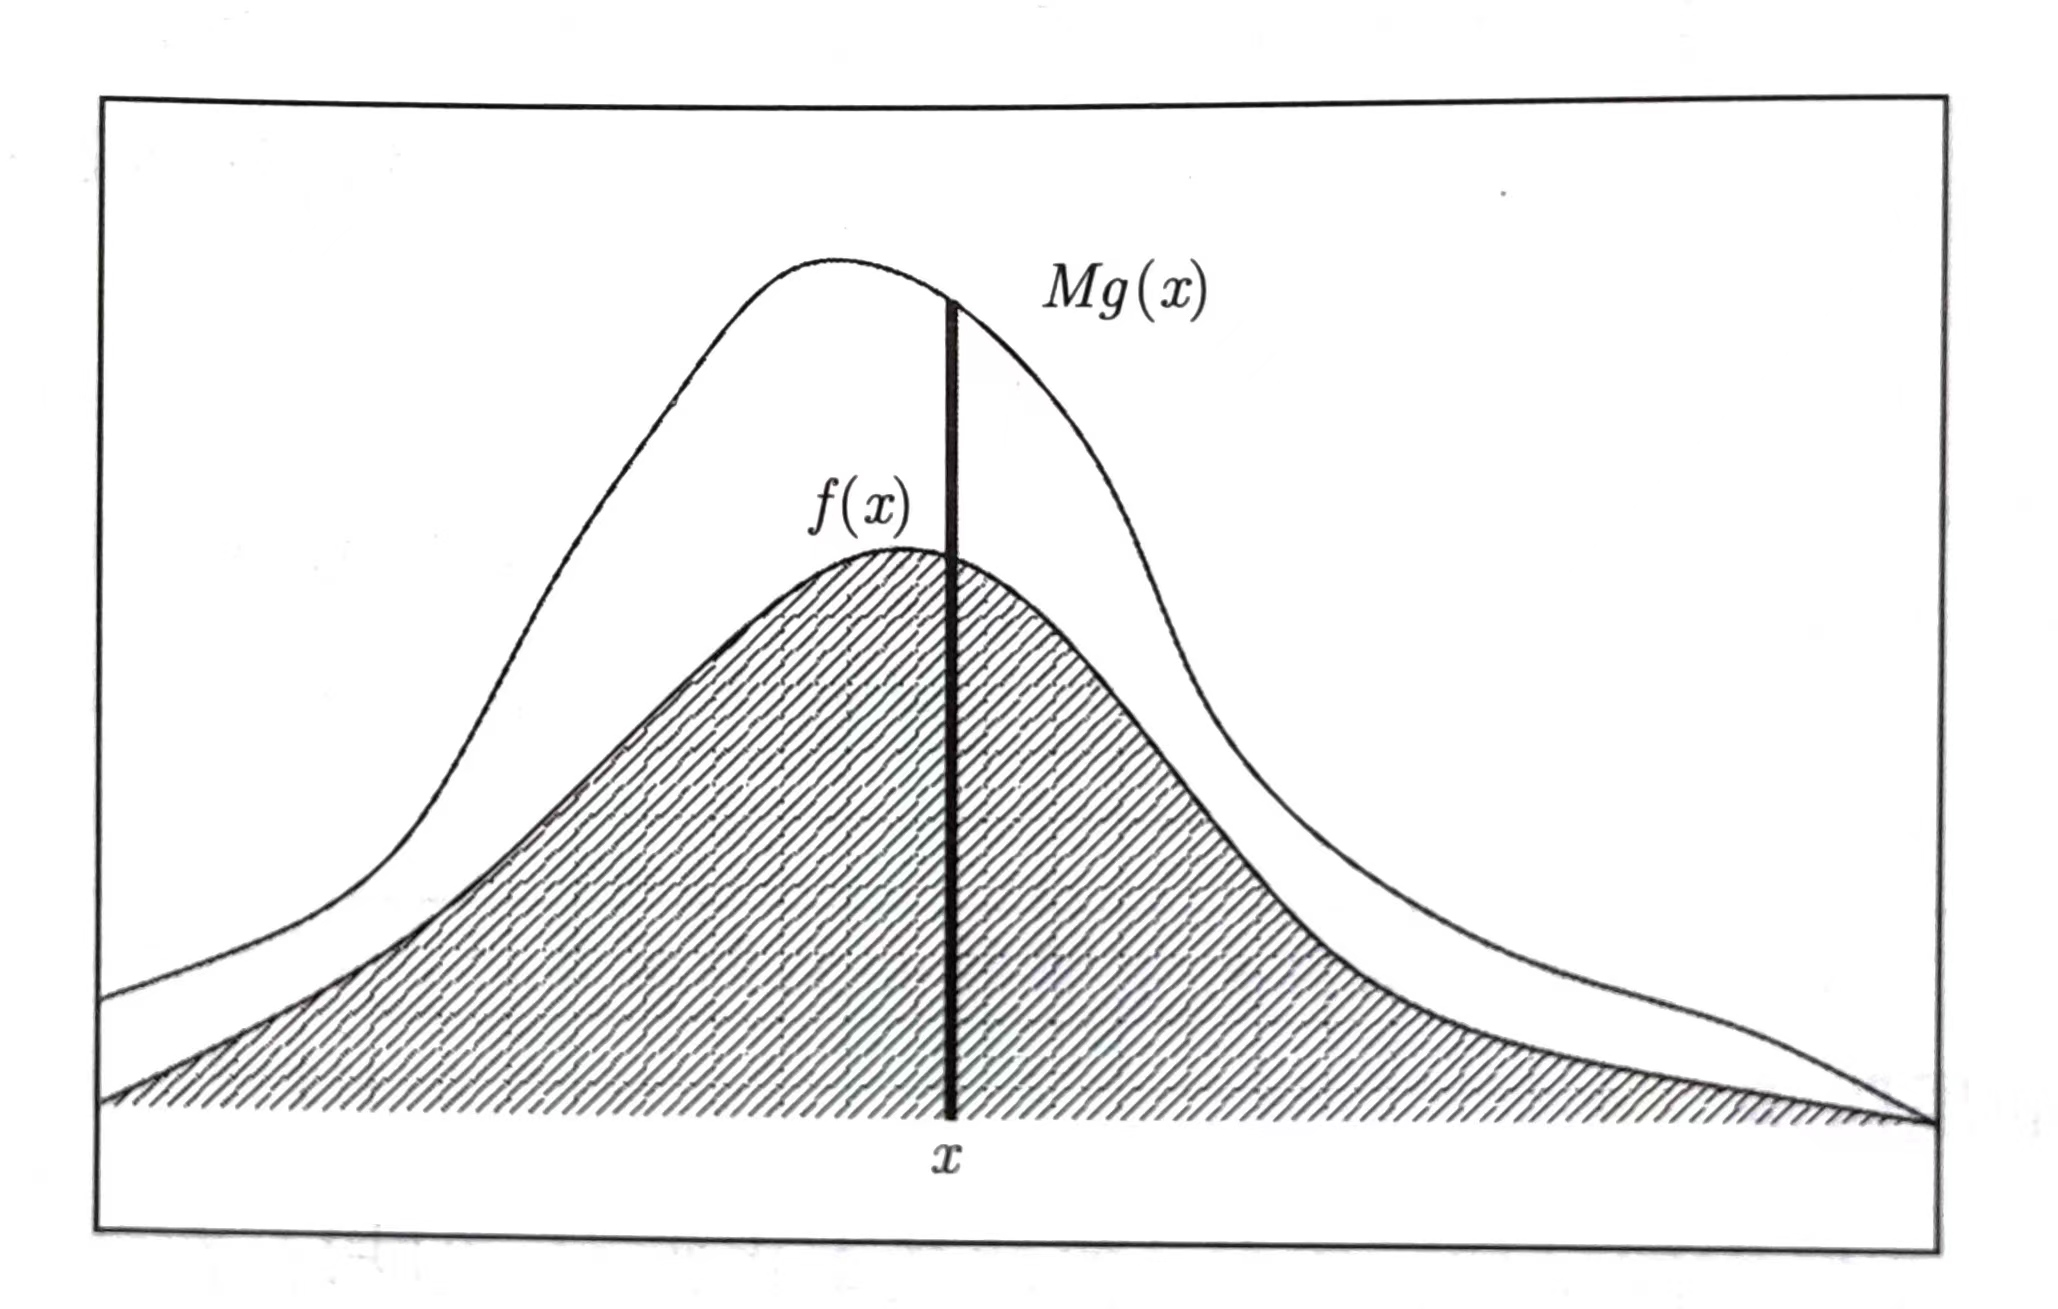
\includegraphics[width = .58\linewidth]{image1.png}
        \end{center}
    \end{figure}

    \begin{itemize}
        \item \(f(x)\): object function
        \item \(g(x)\): proposal function
        \item \(M\): auxiliary constant
        \item Make sure that \(Mg(x)\geq f(x)\) for all \(x \in \Omega\)
    \end{itemize}

\end{frame}
\subsection{Algorithm and Proof}
\begin{frame}
    \frametitle{Algorithm}
    \vspace{-\baselineskip}
    \begin{figure}
        \begin{center}
            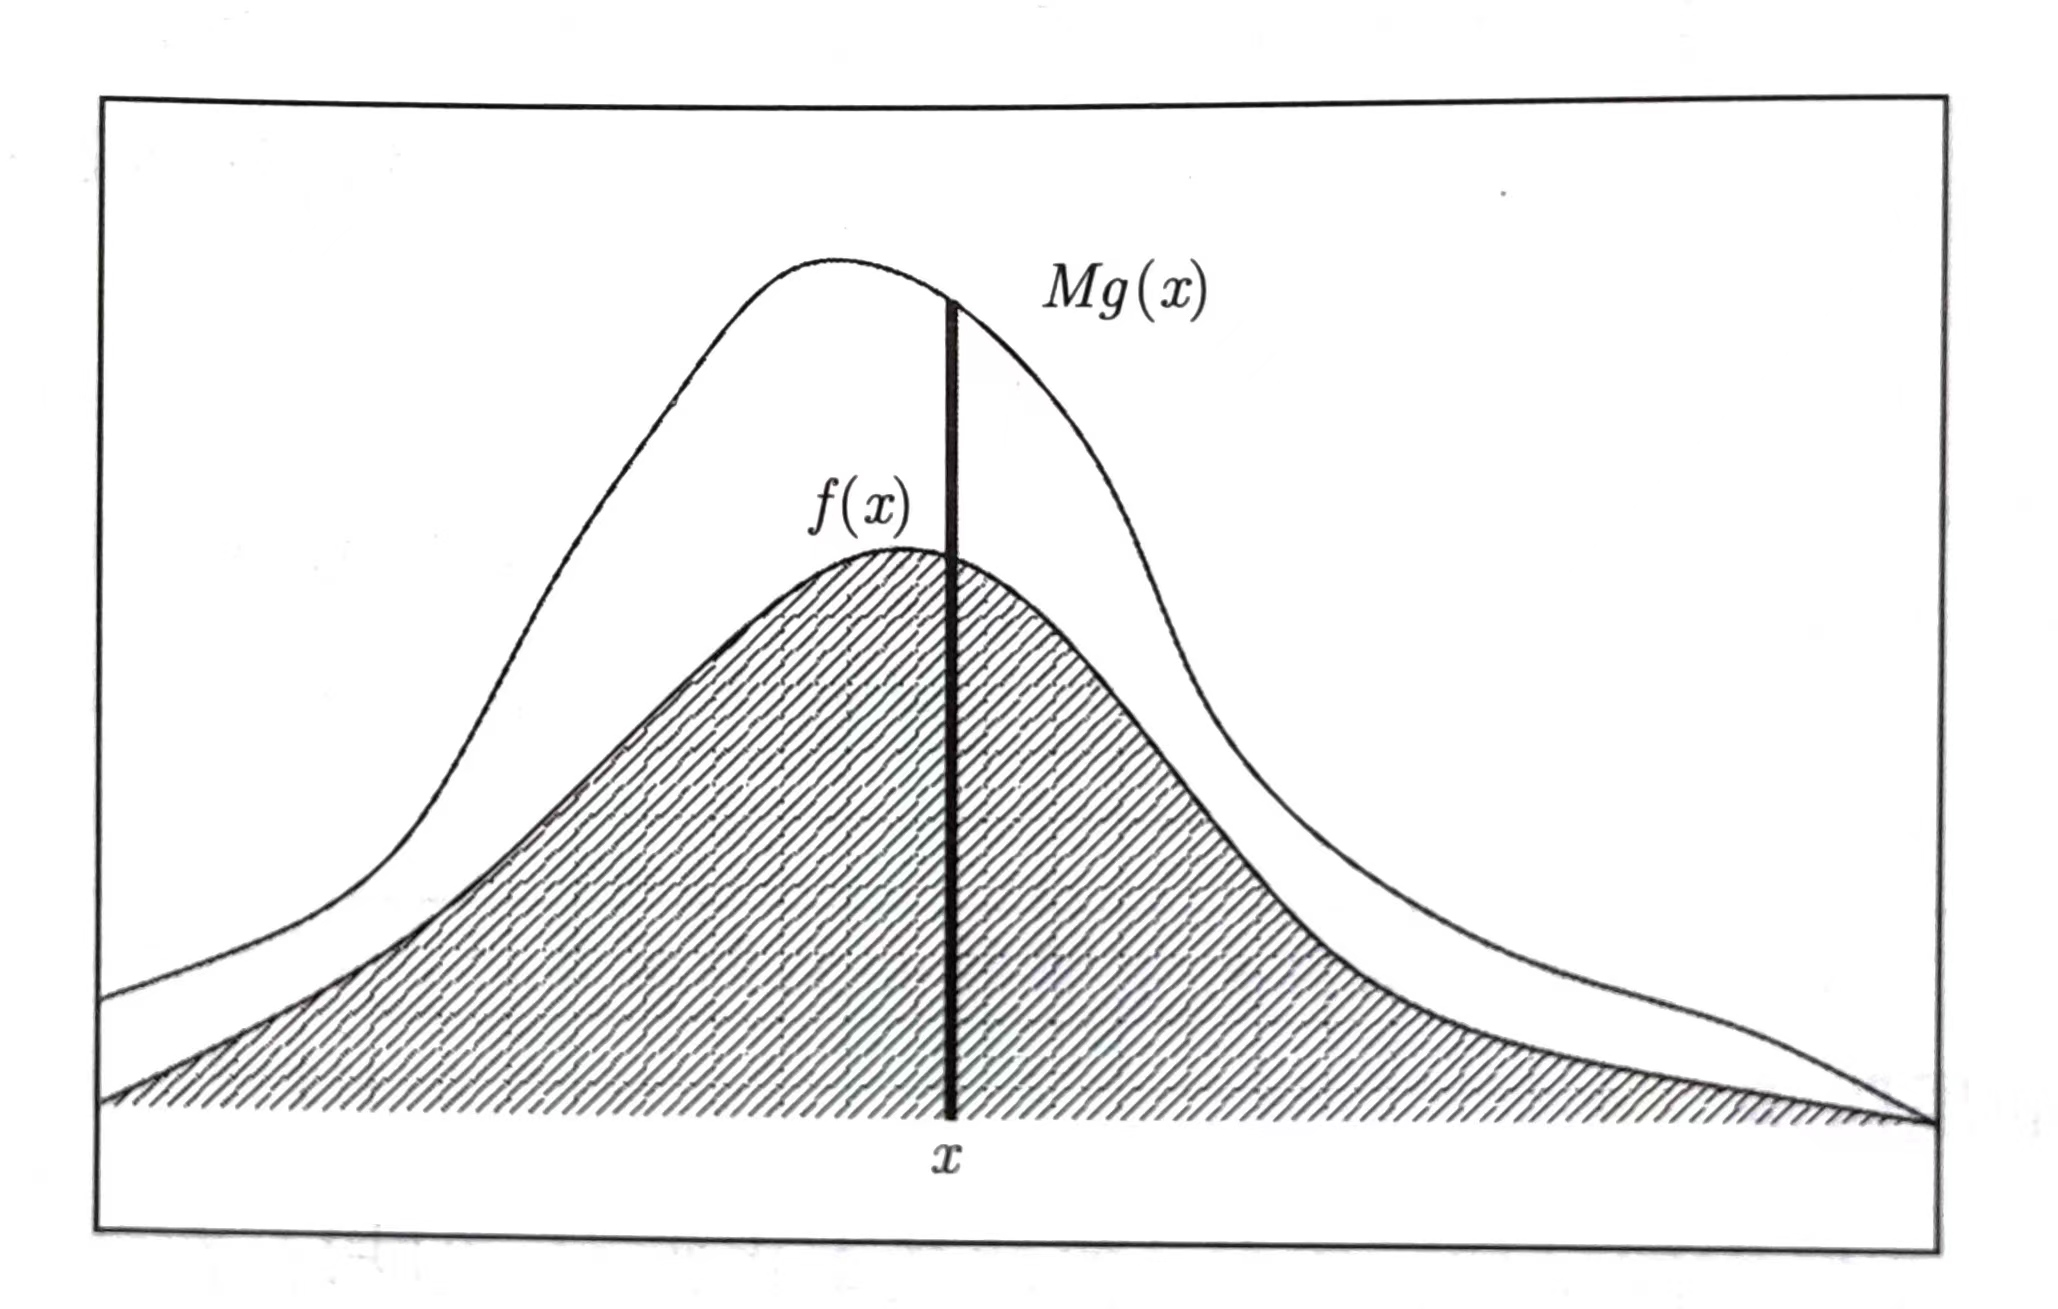
\includegraphics[width = .58\linewidth]{image1.png}
        \end{center}
    \end{figure}
    \vspace{-\baselineskip}
    \begin{enumerate}
        \item Produce a sample \(y\) from \(g(\cdot)\)
        \item Produce a sample \(u\) from \(\operatorname{Unif}(0,1)\)
        \item Do comparasion. If \(u \leq \frac{f(y)}{Mg(y)}\), accept the sample. Otherwise, reject the sample.
        \item Back to the first step unless we already have enough sample.
    \end{enumerate}

    

\end{frame}

\begin{frame}
    \pause
    \frametitle{Proof of Algorithm}
    Let \(U \sim \operatorname{Unif}[0,1]\) and \(Y\) owns PDF \(g(\omega) = F'(\omega)\), one obtain:
    % \vspace*{-.5\baselineskip}
    \begin{align*}
        P\left(U \leq \frac{f(Y)}{Mg(Y)}\bigg |Y = y  \right) = \frac{f(y)}{Mg(y)}
        % \vspace*{-.5\baselineskip}
    \end{align*}
    \pause
    % \vspace*{-.5\baselineskip}
    The total probability is:
    \begin{align*}
        P\left(U \leq \frac{f(Y)}{Mg(Y)} \right) &= \int _{-\infty}^\infty\frac{f(y)}{Mg(y)}g(y) dy = \frac 1 M
    \end{align*}
    \pause
    % \vspace*{-.5\baselineskip}
    By Bayesian's formula,
    \begin{align*}
        &\quad P\left(Y = y \bigg | U \leq \frac{f(Y)}{Mg(Y)}  \right)= P(A|B) = \frac{p(B|A)P(A)}{P(B)}\\
        &= M\int_{-\infty}^ y  P\left(U \leq \frac{f(Y)}{Mg(Y)}\bigg |Y = \omega \leq y  \right)g(\omega) d \omega\\
        &= M\int_{-\infty}^ y   \frac{f(\omega)}{Mg(\omega)} g(\omega) d\omega = F(y)
    \end{align*}

    

\end{frame}

% \begin{frame}{Algorithm}<presentation:0>
%     \scriptsize
%     \begin{algorithm}[H]
%         \KwData{this text}
%         \KwResult{how to write algorithm with \LaTeX2e }
%         initialization\;
%         \While{not at end of this document}{
%             read current\;
%             \eIf{understand}{
%             go to next section\;
%             current section becomes this one\;
%             }{
%             go back to the beginning of current section\;
%             }
%         }
%         \caption{How to write algorithms
%         (copied from \href{https://en.wikibooks.org/wiki/LaTeX/Algorithms}{here})}
%         \end{algorithm}
% \end{frame}
\subsection{Code Implementation}
\begin{frame}[fragile]
    \frametitle{{An Implementation of the Algorithm in R}}
    \framesubtitle<overlay specification>{f(y) = 6 * (y - 0.5)^2 / 7}
        \begin{lstlisting}{language = r,caption={An Implementation of the Algorithm in R}}
N <- 50000
M <- 3.858
y <- runif(N, min = 0, max = 2)
u <- runif(N, min = 0, max = 1)
gy <- 0.5
fy <- 6 * (y - 0.5)^2 / 7
x <- y[u < fy / gy / M]
sample <- length(x)
hist(x, breaks = 50, freq = FALSE, col = "#adabab",
main = "f(x) = 6(x - 0.5)^2/7")
curve(6 * (x - 0.5)^2 / 7, from = 0, 
    to = 2, add = TRUE, col = "red")
    \end{lstlisting}


\end{frame}

\begin{frame}
    \frametitle{Output}

    \begin{center}
        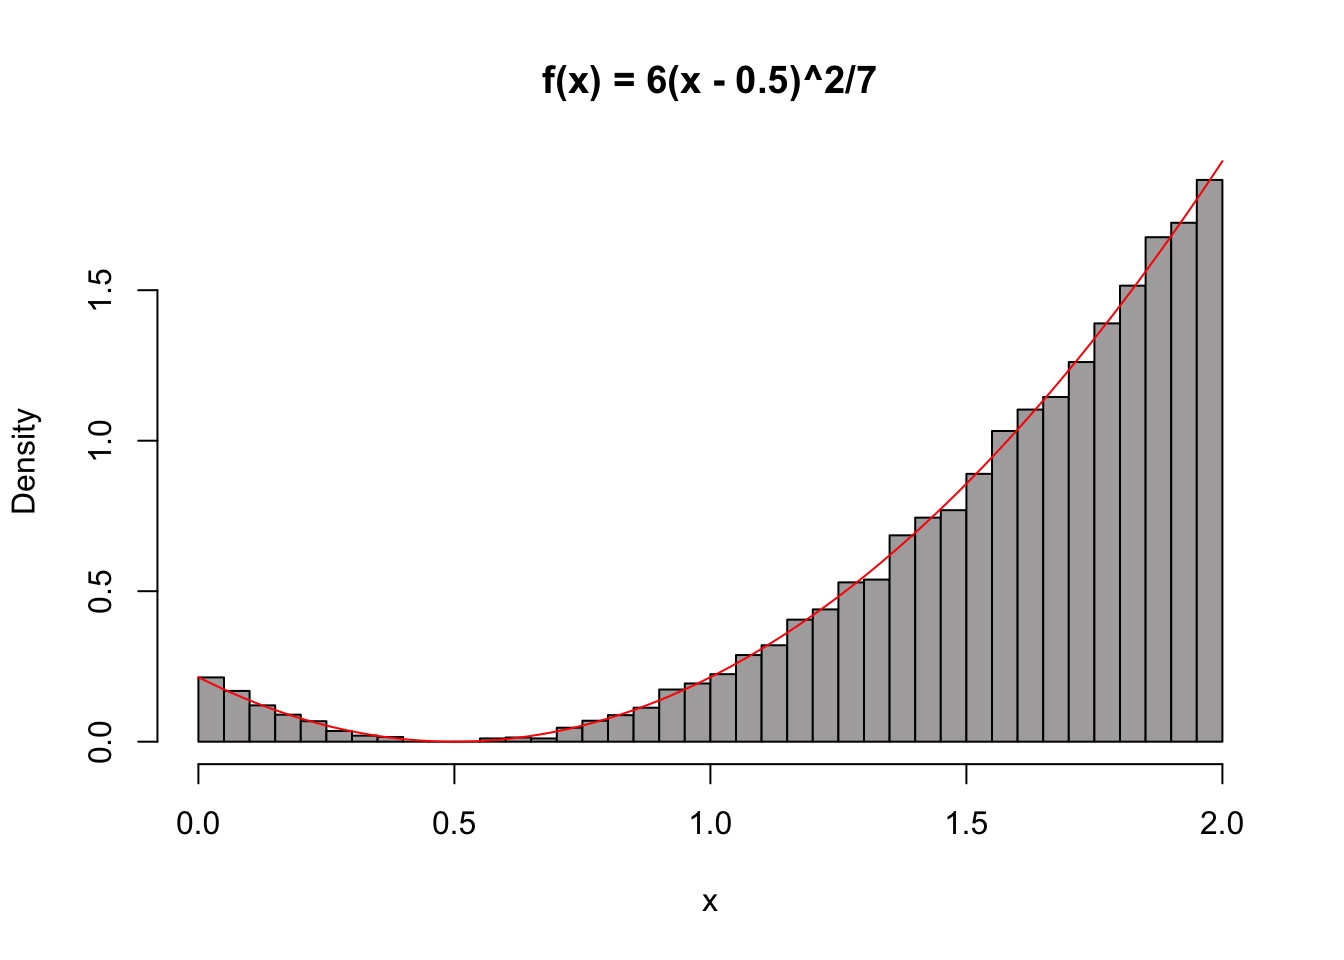
\includegraphics[width = .9\linewidth]{image2.png}
    \end{center}

\end{frame}

\begin{frame}
    \frametitle{Pros and Cons}
    \begin{columns}
        \column{0.5\textwidth}
        \begin{block}{Pros}
            \begin{itemize}
                \item Deal with almost every distribution.
                \item Easy to handle.
            \end{itemize}
        \end{block}
        
        \column{0.5\textwidth}
        \begin{block}{Cons}
            \begin{itemize}
                \item Lack of efficient.
                \item Do not perform perfectly with unbounded PDF, i.e. Beta distribution.
                \item Do not work well with PMF.
            \end{itemize}
        \end{block}

        
    \end{columns}

    

\end{frame}

\section[MCMC]{Markov Chain Monte Carlo Algorithm}
\subsection{Background Knowledge}

\begin{frame}{Background}
    Property of Markov Chain:
    \begin{itemize}
        \item \(P(X_n = x_n |X_{n-1} = x_{n-1}\cdots X_{1} = x_1) = P(X_n = x_n |X_{n-1} = x_{n-1})\) Next state independent of the past states and only depends on the present state.
        % \item Invertible: If \(X_1,X_2\cdots X_n\) is MC, so do \(X_n,X_{n-1}\cdots X_1\).
        \pause
        \item Homogeneous: Transition matrix is independent with time.
        \item Stationary distribution: \(\pi = \pi P\). Every finite positive homogeneous chain have unique Stationary distribution, which is given by \textit{Perron-Frobenius} theorem. The stationary distribution does not depend on initial distribution.
    \end{itemize}
\end{frame}
\subsection{Metropolis Algorithm}
\begin{frame}{MCMC Sampling: Metropolis Algorithm}
    Suppose we want to generate a group of sample from the object PMF \(f(\cdot)\)
\begin{enumerate}
    \item Initialization: Choose arbitrary value \(x_0\), proposal markov chain with transition probability \(g(\cdot|\cdot)\) and set \(t = 1\).
    \item Generate \(x^*_t \sim P(x^*_t | x_{t-1})\) and \(u \sim \operatorname{Unif}[0,1]\).
    \item Compute \[h(x_{t-1},x^*_t) = \min\left\{1,\frac{f(x^*_t)g(x_{t-1}| x_t^*)}{f(x_{t-1})g(x^*_t | x_{t-1})}\right\}\]
    \item If \(u < h(x_{t-1},x^*_t)\), let \(x_{t} = x_t^*\); Otherwise, let \(x_t = x_{t-1}\)
    \item Let \(t++\). Back to the second step unless reach stationary distribution.
\end{enumerate}
\end{frame}

% \subsection{Table}

\begin{frame}{Intuition}
    Immigration problem.
    \begin{itemize}
        \item To keep the population ratio stable.
        \item Randomly reject some visa with specific probability.
        \item Finally, reach a balance.
        \item Aribtrary start does not affect.
        \item Dynamic balance.
    \end{itemize}
\end{frame}

\begin{frame}
    \frametitle{Another Example}
    \centering
    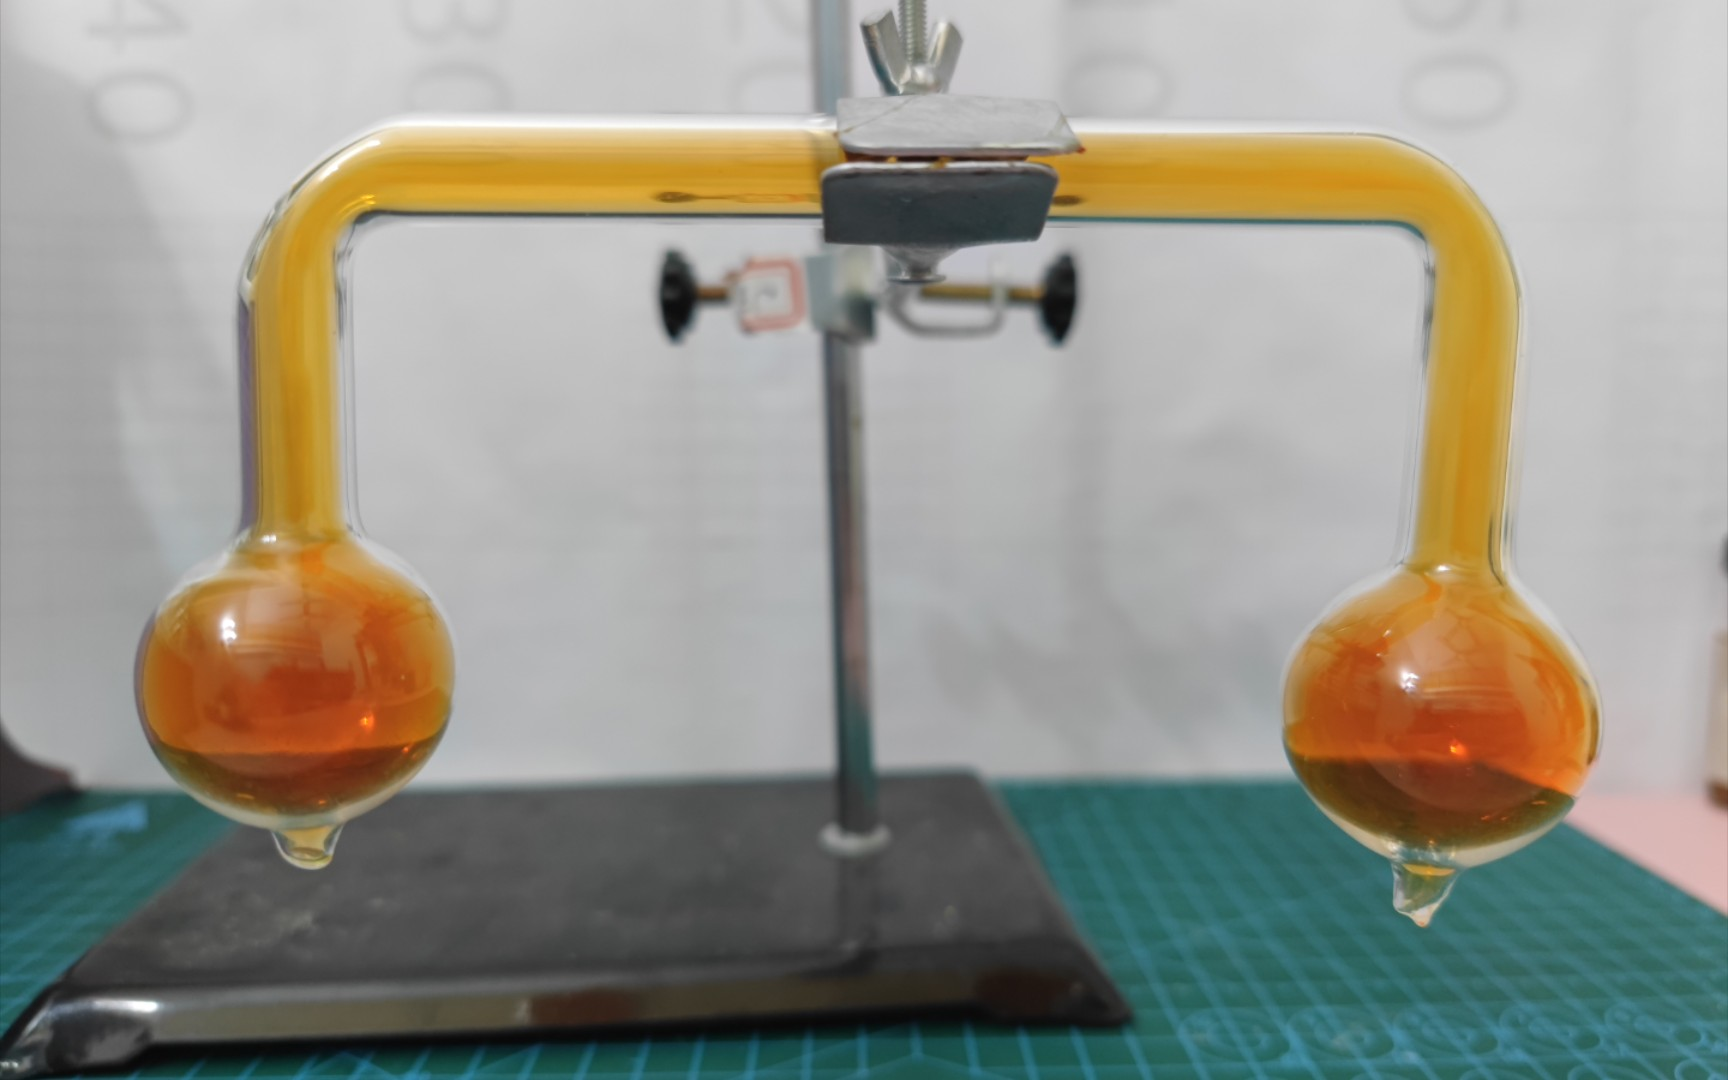
\includegraphics[width = .78\linewidth]{image3.png}

    

\end{frame}

\subsection{Proof of Metropolis Algorithm}

\begin{frame}{Proof of Metropolis Algorithm}
    Detailed balance condition:
    \[\delta_{xy} = m(x)P(x\to y) - m(y)P(y\to x) = 0 \]
    One need to show that \(m(x) \varpropto f(x)\).
    \[\frac{m(x)}{m(y)} = \frac{P(y\to x)}{P(x\to y)} = \frac{h(x,y)}{h(y,x)} = \frac{f(x)}{f(y)}\]

\end{frame}
\subsection{Code Implementation}
\begin{frame}{Simulation: Throwing Two Dice}
    The object PMF is:
    \begin{align*}
        \begin{array}{c|c|c|c|c|c|c|c|c|c|c|c}
            \hline x & 2 & 3 & 4 & 5 & 6 & 7 & 8 & 9 & 10 & 11 & 12 \\
            \hline f(x) & 1 & 2 & 3 & 4 & 5 & 6 & 5 & 4 & 3 & 2 & 1 \\
            \hline
        \end{array}
    \end{align*}
    We apply minimum neighborhood method:
    \begin{align*}
        G=\left(\begin{array}{ccccccc}
            1 / 2 & 1 / 2 & 0 & \cdots & 0 & 0 & 0 \\
            1 / 2 & 0 & 1 / 2 & \cdots & 0 & 0 & 0 \\
            0 & 1 / 2 & 0 & \cdots & 0 & 0 & 0 \\
            \vdots & \vdots & \vdots & \ddots & \vdots & \vdots & \vdots \\
            0 & 0 & 0 & \cdots & 0 & 1 / 2 & 0 \\
            0 & 0 & 0 & \cdots & 1 / 2 & 0 & 1 / 2 \\
            0 & 0 & 0 & \cdots & 0 & 1 / 2 & 1 / 2
            \end{array}\right) .
    \end{align*}

\end{frame}





% \section{Conclusion}

\begin{frame}
    \centering \Huge
    \emph{Thanks}
\end{frame}